\documentclass[10p,letterpaper]{article}

\usepackage{cogsci}
\usepackage{pslatex}
\usepackage{apacite}
\usepackage{graphicx}


\title{The Importance of Interaction in Information Visualization Systems}
 
\author{{\large \bf Matthia Sabatelli (m.sabatelli@student.rug.nl)} \\
  Rijksuniversiteit Groningen\\Department of Artificial Intelligence\\ Nijenborgh 4,
  9747 AG Groningen\\ The Netherlands}

\begin{document}

\maketitle


\begin{abstract}

Cognitive Engineering is the name of a discipline that combines two terms that are very different between each other. On the one side, the first one relates to the world of the human mind and all the processes that guide it, while on the other one, the second term is strongly connected to the development of mechanical and technical techniques that support the creation of technological applications. Although this juxtaposition may seem counter intuitive in this paper I show how a Cognitive Engineering approach is needed when building appropriate Information Visualization Techniques and how this is linked to the importance of developing tools that support interactive processes.       

\textbf{Keywords:} 
Cognitive Engineering, Information Visualization, Interaction, Interactive Techniques, Big Data
\end{abstract}


\section{Introduction}

During the October of 2012 Dr. John Barrett, head of the Embedded Systems Research Center of Cork has given a TED talk in which he estimates that there were almost 4000 exabytes 
of information saved on the cloud. In order to understand the meaning of how large this quantitative of information is, it's possible to correspond this measure to eighty stacks of books that go from the Earth to Pluto. If until fifty years ago academics of all different disciplines were struggling in order to gain some data in order to do their researches on, nowadays this aspect doesn't seem to be an issue any more. Computers and smartphones are only two out of the multiple technological systems that are able to collect information 24/7, information that is safely saved on cloud servers and that due to its incredibly large size has lead to the juxtaposition of the terms \textit{Big \& Data}.\\
If at the one side the problem of collecting information has been solved thanks to the technological developments of the last decades, the formation of Big Data has lead to a likewise dilemma that researchers have to deal with: Information Visualization. Information Visualization, or \textit{Infovis} *Ref*, is a very complex research domain that has as main goal the representation of large-sized information that is mostly saved on the cloud. A lot of research that tries to solve this problem from a pure engineering perspective has been done, computer scientists and engineers have built multiple complex tools and representation strategies that are able to display large amounts of information. However, developing these kind of tools by considering only technical aspects, isn't enough to make the information that is displayed usable and easily understandable to the person who is watching at it. In fact, in order to build a successful information visualization system there is need to understand the cognitive mechanisms that guide the user when it's interacting with the tool, and only in a second moment, by taking these cognitive knowledge into consideration, implementing correct visualization strategies.\\
The main objective of this work is to prove how important it is, to understand the cognitive mechanisms behind the UX of a person that is trying to infer some knowledge from data that is displayed in front of him. In order to do this the paper will be divided into two parts. In the first one an analysis of the overall visualization process will be presented by focusing on how this method relates to some important cognitive science aspects. Once this is done multiple examples of different visualization techniques will be explained. The goal of this part is double, on the one side it aims to present some of the most recent technological achievements that have made it possible to represent large amounts of information, while on the other one, it aims to prove, how large part of the techniques that are considered as successful take into consideration the process of \textit{Interaction}, an aspect that is the link between the digital stored data and the human mind, and that literature doesn't consider as relevant as the pure visualization part.


\section{Insight \& Mental Models}

In this section two important aspects related to the field of cognitive science are presented that both have an impact in the development of Information Visualization System. They are introduced by in *chapter*.\\  
The first concept is defined as \textit{Insight} and is strongly related to the human vision system. Between the five senses, vision is the one that is the most capable of rapid parallel processing and pattern recognition, thanks to the millions of photoreceptors it's in fact possible to acquire large amount of visual information very quickly. However, this isn't enough to understand the data that is presented, the human mind has in fact to deal with a higher level process that leads to the extraction of knowledge from the information that is visualized. If this process turns out to be successful, which means that the user gains some comprehension from the data, it's possible to assert that it has acquired insight. When building a Visualization System this is crucial, in fact, providing the user with insight corresponds to the final goal that \textit{Infovis Systems} have to achieve.\\
The importance of this concept has also been underlined in work *DefiningInsitforVisualAnalytics* where the authors argue that the purpose of visualization is indeed insight, and that appropriate visualization tools should enable the user to discover this concept. However, the authors also highlight the fact that the scientific community has been slow to build on this idea and a commonly accepted definition doesn't exist yet. In order to solve this issue, the paper presents two different definitions of the concept that both have to be taken into account in visual analytics. The first one takes inspiration from the standard cognitive science explanation of the concept and defines insight as the moment of enlightenment that leads to a state in which it's possible to solve a problem that previously was unsolvable. The second one sees insight as a simple advance of knowledge and gain of information. Both definitions turn to fit perfectly to a scenario of a system that is displaying some data to a user that has to understand it, in fact an appropriate visualization tool shouldn't take too long to lead the user to the moment of enlightenment and should do this by providing him with a new piece of information.\\
In order to subsidize the user to get insight a second concept presented by the **chapter** turns to be relevant, it regards \textit{Mental Models}. According to *MentalModelsConceptsRevisited* a Mental Model is a personal explanation of someone's thought process about how something works in reality. In fact, it can be defined as an internal representation of the surrounding world that helps humans to understand a particular phenomenon. According to *chapter* Mental Models turn to be very important in information visualization since the data that is displayed should be in line with the internal mental models of the users, only if this is the case the users will get insight about the data.\\
The importance of understanding the Mental Models of the users in order to facilitate the use of visualizations has also been pointed out in work *MentalModels,VisualReasoningndInteraction*. In this paper the authors assert that most of the current research in \textit{InfoVis} is focused on external visualization and almost no research at all has been done on internal representations. The development of appropriate visualization tools has to deal with the understanding of the internal visualization skills of the users that are as important as the creation of external graphical displaying methods.\\
 	
\section{The Design Process \& The Visualization Pipeline}

Considering the previous two concepts ** in work ** has defined the General Design Process that should be followed when building an Information Visualization Technology. The first aspect that has to be considered when showing information, and that should guide the whole procedure, is related to the mantra of not misleading the user while it's looking at the data that is displayed. This means that the information that is presented has to lead the user to the correct insight by considering its mental models. Moreover, it's also important to verify that the data that is shown is in line with the real structure of the dataset, the visualization of the information has to be coherent with the actual dataset. In order to satisfy this requirement and build an appropriate \textit{InfoVis System} three main steps have been identified:

\begin{itemize}

\item Requirement Analysis Phase: Is the first step of the design process and has a double goal. The first one regards the study of the characteristics of the information that has to be visualized, without knowing the structure of the dataset it's in fact impossible to choose an appropriate visualization technique. However this isn't the only reason that guides this decision, it's also very important to identify which type of insight has to be transmitted to the users and which mental model the dataset has to refer to.
\item Design of the System: Once the previous phase is satisfied it's in fact possible to start building the system by choosing the hardware characteristics that will support the type of representation technique that will represent the data and implementing the software that will display the data. 
\item Evaluation: Is the phase that has as main objective the collection of feedback about how the system works, multiple usability testing techniques developed by UX designers can be used, however it's important to don't keep this phase at the very end of the whole design process. Multiple evaluation tests should guide the creation of a visualization tool in different moments, this is done in order to identify potential problems as soon as possible and avoid any waste of money and resources.  

\end{itemize}  

The General Design Process can be considered as a good starting point, however in order to understand how it's possible to convert information into a visual form properly and more in detail ** , proposes a model that aims to describe this computational process called \textit{Visualization Pipeline} divided in 4 steps. The structure of it is presented in the figure hereafter before the explanation of the procedure:

\begin{figure}[ht!]
\centering
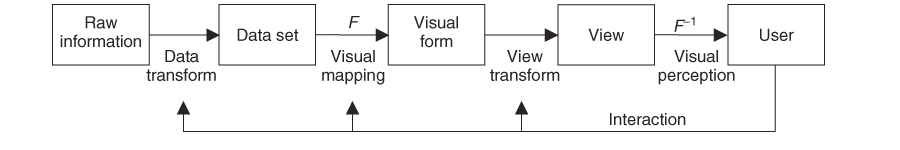
\includegraphics[width = 1.0\linewidth]{/home/matthia/Desktop/pipeline.png}
\caption{The Visualization Pipeline \label{pipeline}}
\end{figure}

\begin{itemize}

\item Phase 1: The first step aims to transform the dataset that has to be visualized into a well-organized canonical data format. Especially when dealing with large amount of information it's very unlikely that the dataset is already in a form that makes it possible to visualize it, in order to face this issue some preprocessing is needed. The final result of this process is obtaining a set of data that has for each entity  a relative attribute.   

\item Phase 2: This step is considered as the heart of the whole visualization process and special attention should be put when approaching it. The goal of this phase is to convert the preprocessed data obtained by the previous step into a visual form containing glyphs that represent the dataset entities. Usually this is done by using particular mathematical functions that get the preprocessed dataset as input and generate a visual representation as output. 

\item Phase 3: In this part of the process the preprocessed and transformed dataset is converted into an actual view that finally displays the information that had to be shown.

\item Phase 4: The final stage of the visualization pipeline sees the user interpreting the view and trying to get some insight from it. In order to facilitate this process the user should be allowed to interact during all the previous three phases if he feels that this might help him in interpreting what is displayed.

\end{itemize}


The \textit{Visualization Pipeline} is an excellent example that shows in a very methodical way the different stages that make it possible to convert data into a visual form. On the one side it highlights the existence of technical issues that can be related to the first two phases of the process, while on the other one, it also presents the existence of Interaction during this algorithmic process. As will be explained more in detail in the next section giving the user the opportunity to dynamically change the \textit{InfoVis System} is the clue of building a successful visual interface.\\
Although this concept isn't explicitly highlighted by *author chapter* work *dataknowledgeingvisualiz* takes inspiration from the visualization pipeline model in order to do so and defining the visualization process as a search process. According to the paper, the user, given a particular dataset to be displayed starts by deciding which visualization tools to use for exploring the data, this means experimenting different controls such as styles, layouts and viewing positions. The way he does this depends from how satisfied he is from the whole process and in this case, satisfaction corresponds to having or not gained insight. Interaction can so be seen as one of the main tools that make the user able to understand the data that is visualized, although in the model of figure \ref{pipeline} interaction is mentioned, only work *asasa* considers it such important to define the visualization process on it. 


\section{Examples of Interactive Techniques}

\section{Future Directions \& Conclusion}
possibile collegamento con machine learning

\section{References}

\nocite{ChalnickBillman1988a}


\bibliographystyle{apacite}

\setlength{\bibleftmargin}{.125in}
\setlength{\bibindent}{-\bibleftmargin}

\bibliography{CogSci_Template}


\end{document}
